% TODO
%
% * finish chapter "history"; incorporate: https://en.wikipedia.org/wiki/Contact_improvisation
%
%%%%%%


\documentclass[a4paper]{article}

\usepackage{graphicx}
\usepackage{url}
\usepackage{hyperref}
\usepackage{wrapfig} % wrap text around image

\newlength\mystoreparindent
\newenvironment{leftindent}[0]{
\setlength{\mystoreparindent}{\the\parindent}
\setlength{\parindent}{0pt}
}{
\setlength{\parindent}{\mystoreparindent}
}
\setcounter{tocdepth}{1}

\setcounter{secnumdepth}{0} %% no numbering

\title{Contact Book}
\date{\today}
\author{Christoph Pickl}

\begin{document}

\pagenumbering{gobble}
\maketitle

\begin{center}
	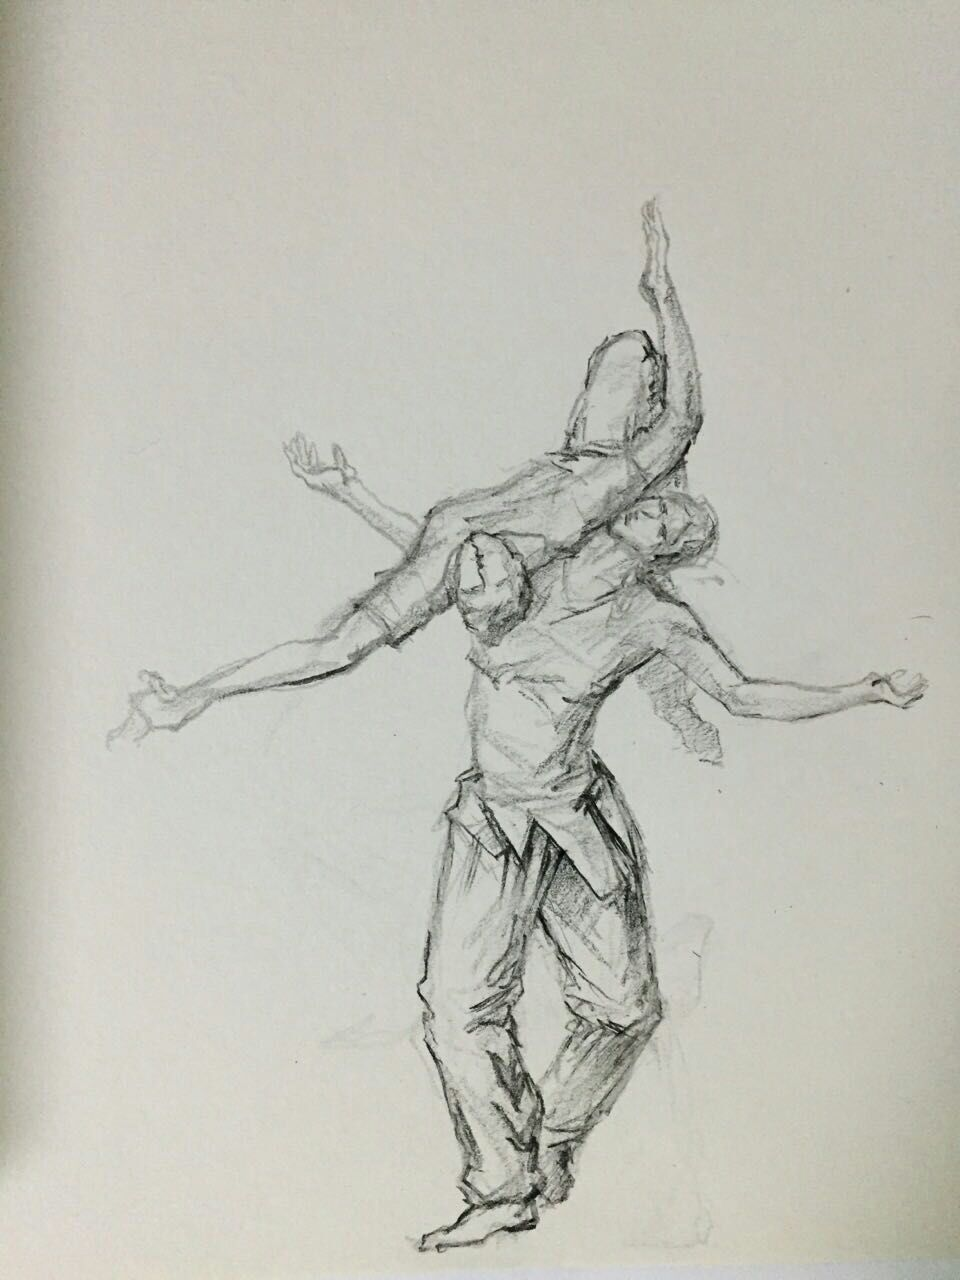
\includegraphics[width=8cm]{images/cover.jpg}
	\vspace{0.5cm}
	
	\textit{Moving in unity.}\\
	\textit{Guided by the moment.}\\
	\textit{In eternal spirals.}
\end{center}
\newpage

\tableofcontents
\newpage

\pagenumbering{arabic}

% TODO: delete "about" chapter, that no other resource AND do use lots of resources (websites, YT videos)

%! prepare lots of good questions; ask tom for an interview; record with phone, and transscript it later, and extract info to put in CI book
% where does CI position itself? dance, movement awareness thingy, therapy, sport,... versus salsa/tango, martial arts, acrobatics?
% saying/hearing yes/no during the dance
% where are its limits/boundaries? what is it not?
% safety. what are the big "no-gos". head above ass.
% sensuality? no... nice, but not here. rolling over frontside?! depersonalize partner, seeing body as physical object, let go of the stories; fall in love with dance not the other dancer.
% netiquette; say your name, ask for name; don't talk too much; proper clothing (no jeans, buttons, ... we were pyjamas)

\section{About}

\begin{wrapfigure}{R}{0.3\textwidth}
\centering
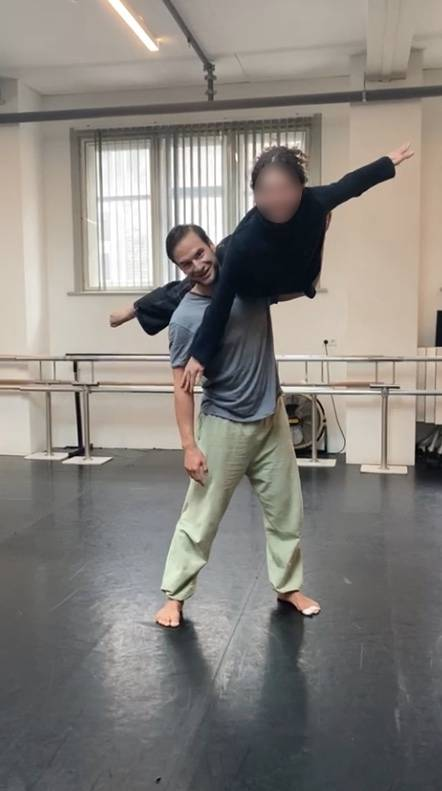
\includegraphics[width=0.25\textwidth]{images/about.jpg}
\end{wrapfigure}

This little book is written by me for taking my personal notes in a digital form, so it might be used by beginners, and non-beginners alike, who are interested in getting more acquainted with the theoretical background of the fine art of Contact Improvisation Dance, or CI for short as of now.

Whatever is written here does not claim to hold any absolute, objective truth, but merely is a manifestation of my own personal, subjective opinions. I deliberately choose not to be too much "influenced" by the work of others, and as such did not read many books or any literature of CI. Instead, I am trying to solely rely on a more "innocent" approach and write about my experiences and interpretation of it, which is of course very much colored by me as a person and my (movement) background.

Speaking of my background: It is mainly Japanese (Karate, Aikido) and Chinese Martial Arts (Taijiquan), and as such, my focus lies more on a practical approach, where "form follows function", and less about any aesthetic aspects as many might consider be an essential part of dancing in a more narrow definition. Furthermore, as a bodyworker (Shiatsu Therapy and Neo-Tantrism), I emphasize the importance of the non-verbal communication aspect of movement and touch. Whether we express ourselves in a free form art or the way we interact with others without words.

For me personally, the looks are irrelevant, and "right" is what is pragmatic, meaning efficient in time and space (thinking of physics, anatomy and biomechanics), and as well whatever is in alignment with the principles of CI. Besides those more physical aspects, the psychological aspect should be granted at least half of the attention: The benefit for one's mental health, the ability to get to know oneself and others more deeply, and of course a more philosophical/spiritual path which can also be walked with the help of this deep art.
\section{History}\label{sec:history}

\begin{wrapfigure}{R}{0.3\textwidth}
\centering
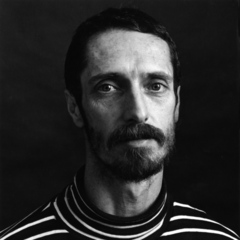
\includegraphics[width=0.25\textwidth]{images/history}
\end{wrapfigure}

In order to know who you are today, I need to know your past, and maybe can even partially predict something about your future.
This applies not only to individuals, but as well to humanity as a whole and localized phenomena like the art of CI itself.
By knowing its origins, we can prevent from diverting too far from it, and reach a deeper understanding of why things the way they are.
And also of course to bring in some kind of attitude of honor, paying our respect to the founding fathers (and mothers).
To bring in some tradition, something our society these days so much lacks and yet so much is in need of (even though it might not be aware of it).

\subsection{Founding Parents}\label{subsec:founding-parents}

CI was developed in June \textbf{1972} in the US by mainly \textbf{Steve Paxton} (``the father of CI'', see picture on the right), which was an American dancer, gymnastics and choreographer (and former Aikidoka, someone who practices the Japanese martial art Aikido) in New York City (Judson Dance Theater).
He wanted to explore and push the boundaries to develop this new practice, some sort of ``art-sport''.

Next to him, it is worth mentioning Nancy Stark Smith (``the mother of CI''), which is the one holding CI still, as Steve stopped doing CI about 7 years after the invention with the intention to giving it to the people.
She continued with another partner and started the Contact Quarterly magazine, a vehicle to share ideas, to hold the theme and practice of CI.

\subsection{Creational Event}\label{subsec:creational-event}

In spring 1972, Steve Paxton invited a group of 17 students and colleagues, dancers, martial artists, acrobats, gymnasts and athletes, to explore and research the \textbf{extremes of movement} and disorientation, from standing still to falling, rolling, colliding and jumping in the air, in a two-week workshop.
While moving with high velocity, running into each other, bumping, trying to survive, and see what the result will be.
A little like what they do in the Large Hadron Collider at CERN, smashing some particles at each other and be excited about what would happen.

He wanted the dancers to work with him on the form he was evolving, and at the end of this week of residency, the group presented a performance named \textbf{Contact Improvisations}.
To see for yourself how the first steps were made, have a look at this old recording: \url{https://www.youtube.com/watch?v=9FeSDsmIeHA}

Out of that exploration, a 20-minutes performance piece called ``\textit{Magnesium}'' arose, whereas the first quarter-hour was about jumping and bumping, manipulation and clinging.
Only the last 5 minutes the so-called ``\gls{smalldance}'' was performed: A form of meditation that is practiced standing, where attention is paid to postural adjustments and micro-weight transfers.
Videos narrated by Steve about that are available, which are very much encouraged to watch, to also see the progression from those impactful years of 72, 75 and 87.

\subsection{Institutionalization}\label{subsec:institutionalization}

At first, around 1975, it was considered to \textbf{trademark} the term contact improvisation, but this idea was rejected in favor of establishing a forum for communication, which nowadays is the online website \url{https://contactquarterly.com}, which is still co-edited by Nancy Stark Smith herself.
So the decision was very deliberate to not have any form of legal institute or certifications, free of any hierarchy.
A certificate usually doesn't mean that that person is good, but just that the certification was passed.

The downside of not having an authority verifying the competence of the teachers is of course that when the word was spreading, more and more injuries started to happen;
that's why one should never teach what one doesn't know properly.

\subsection{Further Spreading}\label{subsec:further-spreading}

A few years after the founding event, 1979, the very first ``Country Jam'' was organized, where 50 people came together to freely exchange and dance, without any structure.
Neither a workshop, conference nor seminar.
Co-created being, dancing and living in flux.
Later on it was introduced in new avant-garde dance schools in the US.

The members of the founding group scattered across the US and started to teach the practice.
It became smoother, continuous and controlled, yet still avoiding eye and direct hand contact.
Much emphasize was put on the experience of flow, which is more of an aesthetic choice (Nancy Stark Smith), yet the central characteristics preserved.

\textbf{Europe} was presented with CI first 1873 in Italy, and later Steve Paxton and Lisa Nelson regularly went to the UK and Amsterdam (School for New Dance Development) as the transmission belts for CI in the whole of Europe.
Belgium was visited by Paxton since the 1980s, but apart certain outbreaks of fever in successful jams, it didn't leave any lasting traces among dancers.

As founding people could be considered (next to Steve Paxton): Nancy Stark Smith, Danny Lepkoff, Lisa Nelson, Karen Nelson, Nita Little, Andrew Harwood, and Ray Chung.

For more detailed information read books like \textit{Sharing the Dance} and others which you can find in the ``\nameref{sec:resources}'' section.

\subsection{Then and Now}\label{subsec:then-and-now}

It was for sure very different back than, which is why also sometimes people would refer to it as ``old school contact'', which some are still doing.
There was a high risk with very high velocity, which for sure looked amazing -and scary.
Good to know though is, that they trained on mats, especially at the very beginning (see videos) which would make the impact of falling much less.
After they started to do the same with mats though, they got (quite a lot of) injuries.

The last few decades much more emphasizes was put on flow (instead on ``explosion''), and also figuring out the least resistant pathway.
Some people claim that CI lost quite a lot of its characteristic along the way, yet it could be said that it's nice to have both, to be able to choose what one wants.
Being able to survive the explosion, and play comfortably in the flow.

Today there are many styles: more flow, more impactful, acrobatics, dance, acting.
The differences are mostly based on the different teachers (lineages) but also due to culturally differences.
Different countries have simply different ``body orientations'', resulting in a different CI style.

\subsection{Future}\label{subsec:future}

Hopefully it will keep a very strong trunk, meaning: People keep on researching the practice, while still knowing where it comes from, knowing its roots.
We are all welcoming the branches, e.g. CI combined with other practices like ``Contact Tango'', ``Contact Beyond Contact'', and so forth; or CI with using substances for ``other states of awareness''.
As the tree is branching, that the main trunk will stay the main trunk, so that there is no need for the distinction between ``I am a CI purist'' but simply say: ``I'm doing CI''.
The last 50 years the trunk stayed stable, yet the last 20 years lots of new branches emerged; branches which merge different forms together.
It is important that people are aware that those branches/merges are not CI the way it is actually practiced.
And lastly, what's needed are good teachers, jams, and spaces where the ideas and principles are held from CI: Knowing the physical aspect but also keeping the history.

% why do it?
\section{Principles}\label{sec:principles}

\begin{wrapfigure}{R}{0.3\textwidth}
\centering
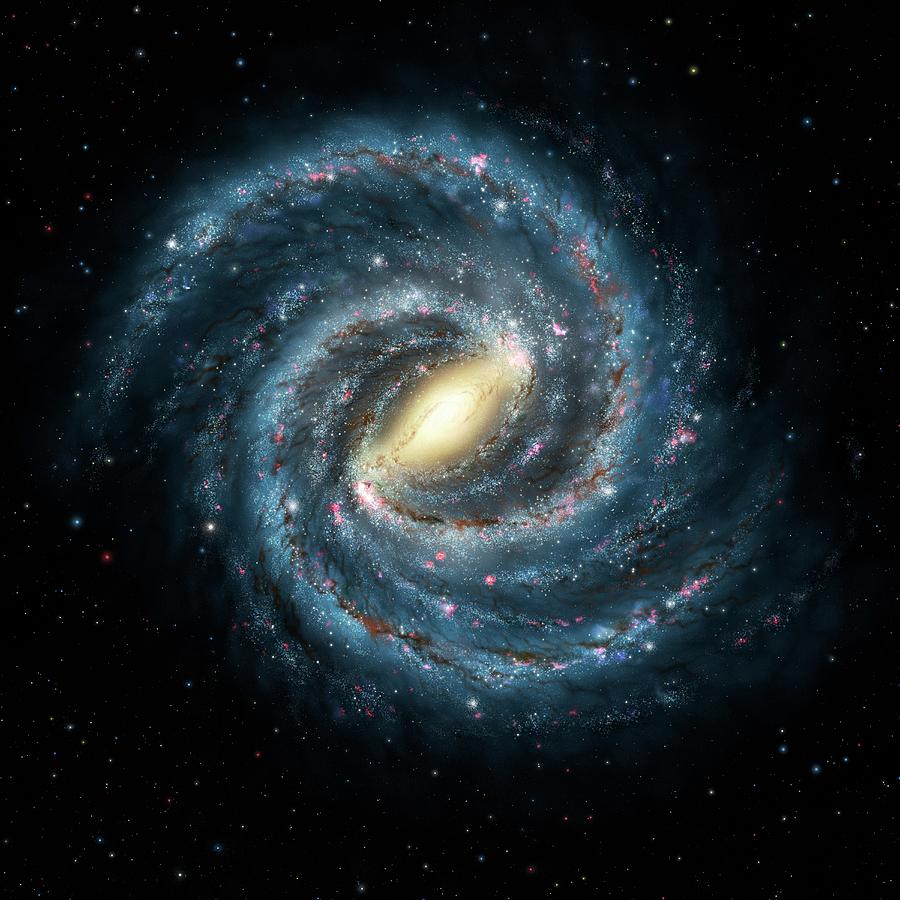
\includegraphics[width=0.25\textwidth]{images/principles}
\end{wrapfigure}

Many systems (sports, martial arts, \...) are focused around dozens or even hundreds of techniques which are thrown at a student to learn by hard, including their names, and precise definitions of what's right and what's wrong.
This is an approach which might work, but obviously has some serious disadvantages when it comes to quickly responding (picking the right technique from many within a split of a second) and more importantly the ability for individual expression.

In contrast to that, CI is centered around a few core principles, and every technique which might be taught, studied and practiced is a manifestation of those core principles.
There are therefore no real moves to be learned, but more principles to be embodied and applied in any given moment.
Once the principles are well understood, one can free oneself from the limitations of specific techniques, and questions like whether something is ``right or wrong'' can be easily answered by asking those principles.
Yet, as it is with the mastery of any art: Once the principles are fully understood, they can be broken if desired so, as: ``\textit{You can do whatever you want, as long as you know what you are doing.}''

\subsection{Grounding}\label{subsec:grounding}

With grounding we are referring to some kind of sensation (light) heaviness in the body, which makes the stance more stable, more robust and thus more connected to the ground.
Imaginary language like ``rooting'', and similar, are often used to describe this internal sensation, with its very realistic impact on the external.
This quality is the beginning of it all, without it we can't go any further, as without a firm foundation there is no house we can build upon it.
To help improving our groundedness we can use visualizations (roots growing into the ground), focusing our attention to where the sole's of the feet have contact with the floor, breathing out and relaxing the muscular tension without collapsing in one's structure, and simply thinking about words which are associated with a grounded, firm, or stable quality.

It should not be confused with stiffness, which so often lead to the illusion of groundedness, which is achieved by simply contracting all muscles; something we don't want to do as it will remove the ability to adapt in the moment, our flexibility.

\subsubsection{Small Dance}

The \gls{smalldance} is a (warming up) exercise helps the practitioner to increase one's body awareness.
It could be considered as some form of mindfulness practice, where we focus our full attention to the sensation of standing; especially of the micro movements in our ankles and whole body.
How some automatic movements, little contractions and twitches, keeping us standing upright.
Something that is beyond our consciousness, but something we can definitely tap into by being more sensitive to it.
We can use these unconscious micro movements as a source of movement by amplifying it.

It is also often used as a beginning of a grounding exercise, by shifting the weight, and keeping the center low.
Additionally to that, once the weight was totally shifted to one side, to ``double ground'' oneself to have a very clear sensation of stability and balance.

\subsection{Pouring Weight}\label{subsec:pouring-weight}

Once we have established to ``gain some weight'' by grounding, we can use that to pour it into another person's body.
The emphasis here is to slowly increase the amount of pressure where the body's have contact, instead of a quick and sudden shift, which will be difficult and fear evoking movement for your partner; ultimately even potentially dangerous.
Instead, we want to ``announce'' that there is some weight approaching, so that our partner can adjust and adapt posture and internal tension/structure to that poured weight.

\subsection{Sharing Weight}\label{subsec:sharing-weight}

The first and most important principle is trying to seek a deep connection between two bodies, sometimes also called ``\textit{umpf}''.
It is different from actively pushing with muscular force, and also different from leaning by which one shifts one's center of gravity beyond a point of no-return.
The sensation should lead to a feeling of the ground beneath the partner's feet.
The body is stable and grounded, yet its limbs and joints are soft and relaxed; like an iron stick wrapped in cotton wool.
The ultimate goal is to maintain this quality throughout (almost) all time.

\subsection{Rolling Point of Contact}\label{subsec:rolling-point-of-contact}

Instead of sliding or jumping (point of contact), by using a spiraling and rotating movement pattern, the contact (and amount of pressure) is always maintained and follows a predictable trajectory, which means both partners can anticipate the very next movement, which furthermore leads to a more ``fluid sensation'' in the dance.
For this to happen, it is required to have a more agile body, bulging out body parts and bending and flexing whenever necessary.

\subsection{Pathway Continuation}\label{subsec:pathway-continuation}

According to the physical law of inertia, and to be in accordance with it, we should never break an already moving momentum (exceptions for the master applied here).
Once spiraling in one direction it should be maintained; possibility for anticipation, predictability and therefore trust on a psychological level, but also a mere reason of energy efficiency on the physical level.

\subsection{Movement Patterns}\label{subsec:movement-patterns}

Through a heightened awareness of communication through movement, touch and sharing weight, we explore the space and the connection between through mutual physical cooperation.
Fundamental movement patterns are:

\begin{itemize}
    \item \textbf{Yielding}: softening/surrendering into incoming force or to gravity
    \item \textbf{Pushing}: expansion, taking up space
    \item \textbf{Reaching}: physically or meta-physically
    \item \textbf{Pulling}: contraction, up til collapsing
    \item \textbf{Releasing}: relaxing into what's contracted before
\end{itemize}

All of those movements can be done easily with little muscular effort if basic physical forces are acknowledged and taken advantage of, such as: gravity (falling), momentum, inertia, balancing and others.
And all of those while staying in contact.

\subsection{Relaxation}\label{subsec:relaxation}

We move usually rather relaxed; a body which is ready for action yet open for receiving tactile stimulus, open for information.
We try to achieve that by deep breathing, by keeping a fluid movement quality (``octopus quality'') and also avoid a staring eye gaze.

Yet, a relaxed state should not be confused with a collapsed one.
An active state is also not the same as a hyper-tensed one.
Within this spectrum of non-extremes, we ought to find the optimal amount of muscle tonus which is appropriate for a given situation.

% zoo; famous animals (little animal, panda, octopus)
% guidelines/mottos: tension (masks sensation), breath, eyes
% techniques: lifts, spirals
% vocabulary: umpf, botsen, wee

\end{document}

